\documentclass[12pt,a4paper]{article}
\usepackage{fontspec}
\setmainfont{Arial}
\usepackage{polyglossia}
\setdefaultlanguage{ukrainian}
\setotherlanguage{english}
\usepackage[a4paper,margin=2.2cm]{geometry}
\usepackage{graphicx}
\usepackage{booktabs}
\usepackage{longtable}
\usepackage{array}
\usepackage{float}
\usepackage{hyperref}
\usepackage{xcolor}
\usepackage{fancyhdr}
\usepackage{titlesec}
\definecolor{navy}{HTML}{17233B}
\definecolor{blue}{HTML}{3D68ED}
\definecolor{light}{HTML}{F2F5FA}
\definecolor{muted}{HTML}{667085}
\hypersetup{colorlinks=true,linkcolor=blue,urlcolor=blue}
\titleformat{\section}{\Large\bfseries\color{navy}}{}{0pt}{}
\titleformat{\subsection}{\large\bfseries\color{navy}}{}{0pt}{}
\pagestyle{fancy}
\fancyhf{}
\lhead{\small Sports Events NoSQL Lab}
\rhead{\small Лабораторна робота №2}
\cfoot{\thepage}
\setlength{\headheight}{15pt}

\begin{document}

\begin{titlepage}
\centering
\vspace*{2.5cm}
{\color{blue}\Large ЛАБОРАТОРНА РОБОТА №2\par}
\vspace{0.8cm}
{\color{navy}\Huge\bfseries NoSQL у системі\\[0.2cm] спортивних подій\par}
\vspace{1.2cm}
{\large PostgreSQL, MongoDB, Redis і .NET 8\par}
\vfill
\begin{flushleft}
\textbf{Виконавець:} Кашинський Владислав, група ТТП-32\\[0.4cm]
\textbf{Предмет:} Сучасні технології баз даних\\[0.4cm]
\textbf{Репозиторій:} \texttt{sports-events-nosql-lab}\\[0.4cm]
\textbf{Рік:} 2026
\end{flushleft}
\vfill
{\color{navy}\large GitHub: kashysnkyi/sports-events-nosql-lab\par}
\end{titlepage}

\section{Мета роботи}

Показати практичне використання різних моделей NoSQL у системі спортивних подій. PostgreSQL зберігає нормалізовані дані та транзакційні зв'язки, MongoDB формує денормалізовану read-модель каталогу, а Redis використовується для кешу, лічильників і рейтингу популярності.

\section{Перевірений склад репозиторію}

Репозиторій містить:

\begin{itemize}
\item \texttt{postgres/schema.sql}, \texttt{seed.sql}, \texttt{benchmark-seed.sql} і SQL-еквівалент NoSQL-моделі;
\item \texttt{mongodb/init.js} зі схемою валідації та трьома індексами;
\item \texttt{mongodb/queries.js} з find, text search, aggregation та explain;
\item \texttt{redis/queries.txt} з командами key-value, hash, set і sorted set;
\item .NET 8 застосунок у \texttt{src/SportsEvents.NoSqlLab};
\item \texttt{docker-compose.yml} для PostgreSQL, MongoDB і Redis;
\item \texttt{benchmark/results.json} з відтворюваним результатом вимірювання;
\item \texttt{README.md} і \texttt{REPORT.md}.
\end{itemize}

На момент перевірки основна гілка містила один коміт: \texttt{4cf004a4a374326aa980a0facca214783a801154} від 07.11.2026.

\begin{figure}[H]
\centering
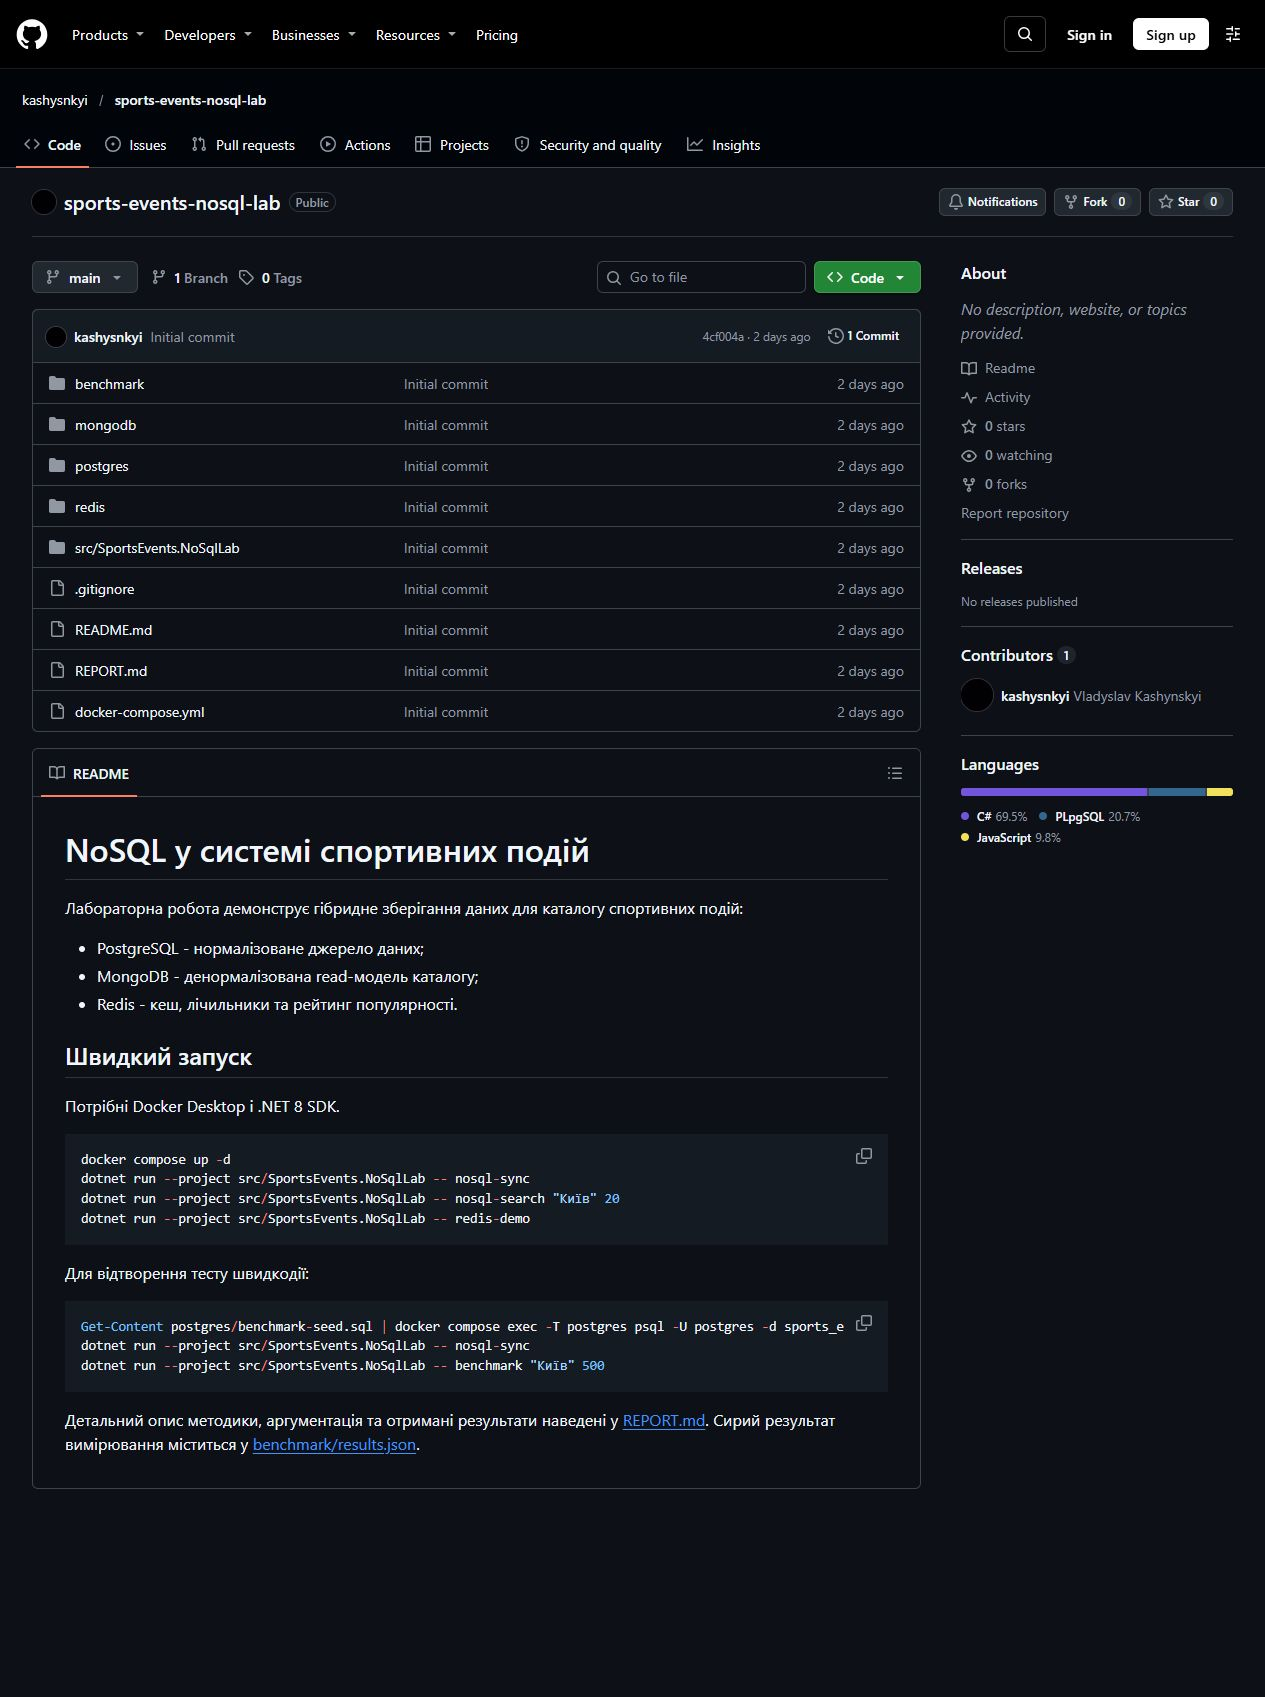
\includegraphics[width=\textwidth]{screenshots/github-repository.png}
\caption{Сторінка репозиторію GitHub і структура лабораторної}
\end{figure}

\section{Архітектура рішення}

\begin{table}[H]
\centering
\small
\begin{tabular}{p{0.25\textwidth}p{0.61\textwidth}}
\toprule
\textbf{Компонент} & \textbf{Роль}\\
\midrule
PostgreSQL & Джерело істини, зв'язки, обмеження, soft delete, реєстрації та SQL-представлення.\\
MongoDB & Колекція \texttt{event\_catalog} з вкладеним спортом, локацією, організатором і категоріями.\\
Redis & Кеш картки події з TTL, hash лічильників, set міст і sorted set популярності.\\
.NET 8 & Синхронізація PostgreSQL -> MongoDB, пошук, benchmark і демонстрація Redis.\\
Docker Compose & Єдиний запуск інфраструктури з трьома сервісами.\\
\bottomrule
\end{tabular}
\end{table}

\section{MongoDB read-модель}

Документ \texttt{event\_catalog} містить поля події та вкладені об'єкти:

\begin{itemize}
\item \texttt{sport} з id і назвою;
\item \texttt{venue} з id, назвою, адресою і містом;
\item \texttt{organizer} з id і назвою;
\item масив \texttt{categories} з кількістю підтверджених реєстрацій;
\item агреговане поле \texttt{confirmedRegistrations}.
\end{itemize}

Синхронізація виконується методом \texttt{ReplaceFromPostgresAsync}: дані читаються з \texttt{sports.v\_event\_catalog\_sql}, колекція оновлюється через bulk upsert, після чого очищаються застарілі документи.

У \texttt{mongodb/init.js} створено:

\begin{itemize}
\item compound B-tree індекс за статусом, містом, датою і id;
\item text індекс за назвою, видом спорту та категоріями;
\item descending індекс за \texttt{lastModifiedAt}.
\end{itemize}

\section{Redis}

Метод \texttt{redis-demo} демонструє чотири структури:

\begin{itemize}
\item \texttt{SET/GET} картки події з TTL 10 хвилин;
\item \texttt{HSET/HGETALL} лічильників переглядів і заявок;
\item \texttt{SADD/SMEMBERS} множини подій міста;
\item \texttt{ZADD/ZREVRANGE} рейтингу популярності.
\end{itemize}

Реалізація використовує \texttt{StackExchange.Redis}. Сценарій не дублює транзакційні дані PostgreSQL, а зберігає короткоживучі похідні значення.

\section{Еквівалент у PostgreSQL}

Файл \texttt{postgres/nosql-equivalent.sql} створює view \texttt{v\_event\_catalog\_sql} і функцію \texttt{fn\_search\_event\_catalog}. View збирає картку події через зв'язки шести нормалізованих таблиць і формує категорії як JSONB-масив.

Таке порівняння показує різницю моделей:

\begin{itemize}
\item PostgreSQL збирає картку під час запиту;
\item MongoDB читає готовий документ без JOIN;
\item дані MongoDB є похідною read-моделлю та потребують синхронізації.
\end{itemize}

\section{Benchmark}

Файл \texttt{benchmark/benchmark-seed.sql} створює 10 000 подій, 30 000 категорій і 360 000 підтверджених реєстрацій. Для вимірювання використано 8 прогрівальних і 500 основних ітерацій. У кожній ітерації перевіряється не лише кількість, а й множина id результатів.

\begin{table}[H]
\centering
\small
\begin{tabular}{p{0.26\textwidth}rrrrr}
\toprule
\textbf{Сховище} & \textbf{Mean} & \textbf{Median} & \textbf{P95} & \textbf{Min} & \textbf{Max}\\
\midrule
PostgreSQL, мс & 33.831 & 39.041 & 50.440 & 14.111 & 60.747\\
MongoDB, мс & 2.109 & 1.588 & 4.188 & 0.804 & 40.275\\
\bottomrule
\end{tabular}
\end{table}

Обидва сховища повертали однакові 50 id подій. У цьому конкретному read-heavy сценарії MongoDB мала середню затримку у 16.04 раза меншу. Це не означає загальної переваги MongoDB: PostgreSQL залишається джерелом істини для транзакцій, унікальності та зв'язків.

\begin{figure}[H]
\centering
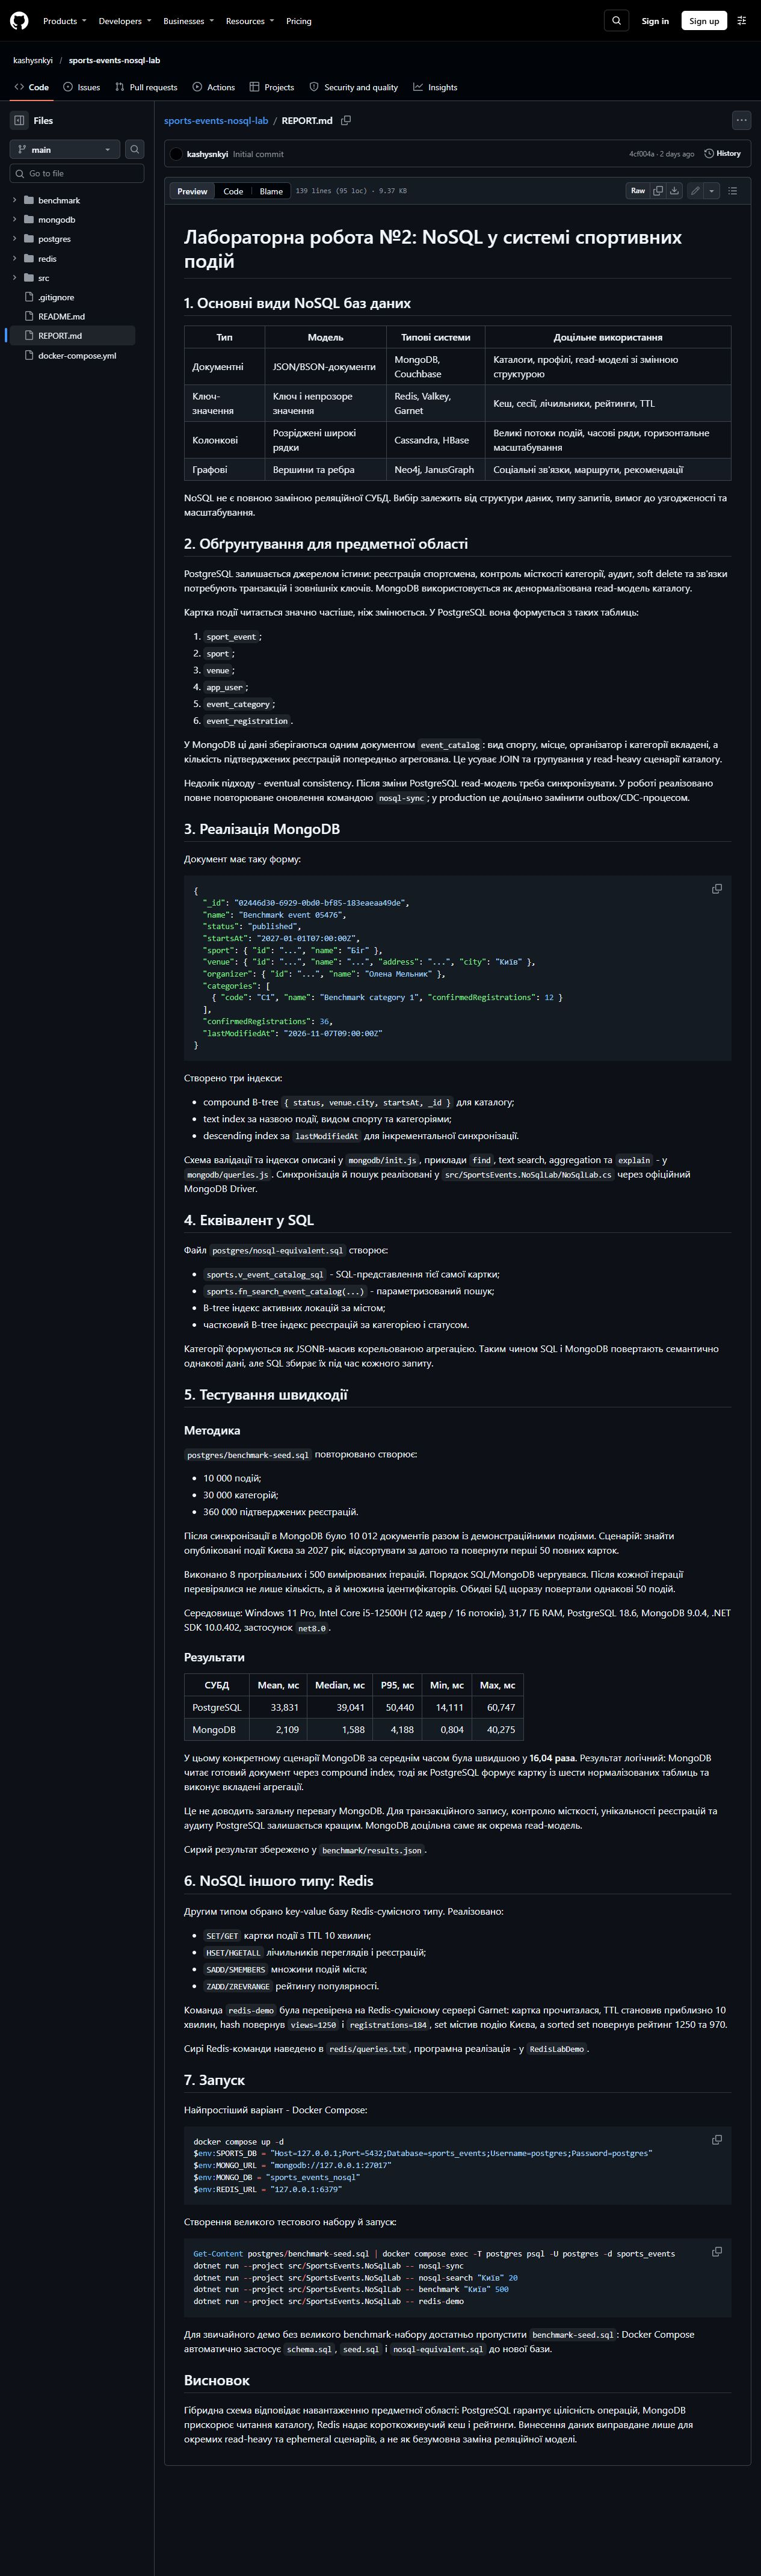
\includegraphics[width=\textwidth]{screenshots/github-report.png}
\caption{Файл REPORT.md з описом методики та результатів}
\end{figure}

\section{Перевірка працездатності}

Виконані перевірки:

\begin{enumerate}
\item Репозиторій клоновано з GitHub, структура файлів перевірена.
\item Проєкт .NET 8 зібрано командою \texttt{dotnet build --configuration Release}: 0 помилок і 0 попереджень.
\item Команду довідки застосунку запущено успішно: доступні \texttt{nosql-sync}, \texttt{nosql-search}, \texttt{benchmark}, \texttt{redis-demo}.
\item \texttt{benchmark/results.json} перевірено на узгодженість: 500 ітерацій, 50 результатів з кожної БД, speedup 16.044.
\item У текстових файлах не виявлено небажаних згадок про генератори або сторонні інструменти.
\end{enumerate}

Повний інтеграційний запуск Docker у цьому середовищі не виконувався, оскільки Docker CLI недоступний. Файли Compose, SQL, MongoDB init-скрипт і .NET-код перевірені статично, а компіляція .NET пройшла успішно. Для очної демонстрації достатньо запустити Docker Desktop і команди з \texttt{README.md}.

\section{Висновок}

Друга лабораторна реалізована як гібридна NoSQL-система. PostgreSQL зберігає узгоджені нормалізовані дані, MongoDB прискорює читання каталогу через денормалізовану модель, а Redis обслуговує кеш та рейтинги. Репозиторій містить код, конфігурацію Docker, SQL-скрипти, запити, benchmark і документацію. Перевірка збірки та контрольних результатів пройшли успішно.

\end{document}
